% \comment{
%     Introduction to declarative programming \& coordination languages
%     Introduction to Reo
%     Terminology
% }

This section introduces concepts and terminology relevant for the majority of the sections to follow. In addition to theoretical concepts, the languages \textbf{Reo} and \textbf{Linda} are outlined and they differ significantly from most general-purpose programming languages the reader may be most familiar with.

\subsection{Scaling beyond Moore's Law}
As Moore's law is grinding to a halt, we are forced to move beyond single-computer architectures and develop applications on parallel and distributed systems for greater speedup. This paradigm shift brings new complications to the table such as verifiability of distributed systems, high- and low-level synchronization and correctness. Amdahl's law seeks to represent the scalability of a system by analyzing its speedup capabilities as a function of its non-parallelizable bottleneck. Gustafson's law redefines scalability when problems are allowed to scale up with the infrastructure~\cite{amdahls}. In practice, scalability is hard to achieve, as adding concurrency to a program requires extra consideration of memory access and synchronization patterns. Message passing frameworks such as \textbf{MPI} have been dominating this new era of computing~\cite{MPI}. As argued in Section~\ref{intro}, programmers are required to use primitives developed decades ago, as well as understand the complex execution structure of such a massive system. The new age of computing requires programming languages to facilitate these complex programs.

\subsection{Declarative Languages}
Declarative programming represents a paradigm of expressing computational results without specifying control flow. This approach is relevant for its association with highly concise high-level code as well as lending itself well to formal verification. While theoretical computer scientists are most familiar with these side-effect-free approaches, as they adhere more closely to the logical models with which they work, even fundamentally-imperative languages like C usually rely on declarative auxiliary tools such as \textbf{Make} in their everyday workflows~\cite{makefiles}.

Listing~\ref{lst:prolog} shows a code snippet written in the declarative programming language \textbf{Prolog}, along with an explanation, showcasing the fact-based structure of the paradigm.
% Prolog was one of the first logical programming languages, used for querying relationships based on a set of facts and rules, today it remains one of the most popular languages for this intended purpose. 
\begin{listing}[t!]
\footnotesize
\begin{minted}[breaklines,mathescape,frame=lines,tabsize=4]{prolog}

good(whiskas).
good(milk).
hungry(alice).
likes(alice, milk).
likes(alice, whiskas).
eat(X, Y) :- hungry(X), likes(X,Y), good(Y). 

\end{minted}
\caption{Example Prolog program that declares the relationships between abstract variables and constants. When queried with \mintinline{prolog}{?- eat(X,Y).}, Prolog checks whether there is a substitution for which the expression is \mintinline{prolog}{True}.}
\label{lst:prolog}
\end{listing}
% \begin{listing}[]
% \footnotesize
% \begin{minted}[breaklines,mathescape,frame=lines,tabsize=4]{prolog}
% mother_child(trude, sally).
% father_child(tom, sally).
% father_child(tom, erica).
% father_child(mike, tom).
% sibling(X, Y)      :- parent_child(Z, X), parent_child(Z, Y).
% parent_child(X, Y) :- father_child(X, Y).
% parent_child(X, Y) :- mother_child(X, Y).
% \end{minted}
% \caption{Example Prolog program that declares the relationships between abstract variables and constants. When queried with \mintinline{prolog}{?- sibling(sally, erica)}, the runtime matches the clause head to known rules (recognizing that \textit{sally} and \textit{erica} share a father: \textit{tom}), evaluating the queried fact as{True}.}
% \label{lst:prolog}
% \end{listing}






\subsection{Coordination Languages}

Coordination languages facilitate the cooperation of several components, concurrently working on a task. Often, they manifest as part of a larger tool-chain that offers a high-level means of communication between seemingly-isolated computation `components'~\cite{coordination}. Typically, the coordination code is compiled down to the target language, generating the needed low-level \textit{glue code} automatically. Here, computation and coordination code are entirely entwined.

\textit{Endogenous} coordination languages are characterized by facilitating communication by injecting simple primitives into the target language that the programmer can weave into their code, hence the name meaning `of the inside'~\cite{coordination}. \textbf{Linda} is an example of such a language, providing an abstract notion of some shared-memory data structure called the `tuple-space' which can store and provide tuples of data~\cite{reoLinda, linda}. Linda can thus `lift' sequential code to a component in a concurrent program by providing stub functions that allow it to read or write to the tuple-space. Upon compilation, tuple operations are translated to message-passing primitives. The tuple-space itself is translated to a potentially-distributed memory store across physical nodes~\cite{linda}.

\textit{Exogenous} communication languages prefer to isolate the coordination and computation components from one another, allowing some view `of the outside'~\cite{reoLinda}. This results in a clear place to find the implementation \textit{of the protocol}, while computation code sees only communication endpoints, but not how and to whom they communicate. \textbf{Reo} is such a language, which allows a programmer to translate their protocol to a high-level hypergraph\footnote{Hypergraphs generalize graphs, allowing edges that connect an arbitrary number of vertices.} representation that represents channels or relations between abstract graph nodes~\cite{criticalPathReo}. 
Reo focuses on \textit{interactions} rather than \textit{actions}, coordinating the activity of computational entities such as sequential code, passive or active objects, threads, processes or software components. These entities communicate though connectors. Complex connectors are formed of simpler connectors, ultimately composed of channels~\cite{introReo}. A channel's end-nodes can be either of type `sink' (which supply data from a channel), or `source' (which accept data into a channel)~\cite{proper}. 

A channel describes its behaviour via constraints or relations on the flow of data at its ends (giving the language its name, named after the word `flow' in Greek)~\cite{introReo, criticalPathReo}. There is liberty in defining the behaviour of a channel as well as the possibility to use multiple types together.
% In Reo, protocols are seen as connectors. Its constraint declaratively defines what relations must hold, overlooking how they hold. 

As desired, components can be plugged into the positions of some of these graph nodes. Figure~\ref{fig:reoConnector} illustrates the relationship between connectors, nodes and components. At compile time, the entirety of the system once again compiles down to granular message-passing between these sequential processes in the target language. At time of writing, Reo can target C, Java, C++ and Fortran~\cite{reoLinda, global}.
%Components can be written in C/Java, compilers take care of the merge and binary translation. \cite{proper} 
\begin{figure}
\centering
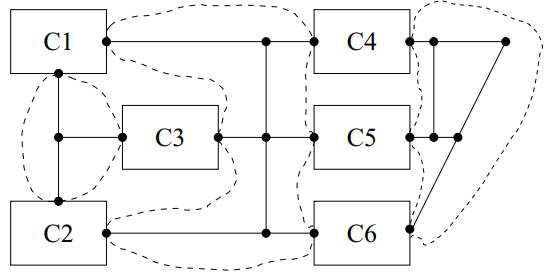
\includegraphics[page=1, width=0.4\textwidth]{images/reoConnector.png}
\caption[]{A system containing compute components $\{C1, C2, ... , C6\}$ with three complex connectors. Each connector is composed of multiple channels, each channel with its own semantics. Image  from~\cite{introReo}.}
\label{fig:reoConnector}
\end{figure}